% Options for packages loaded elsewhere
\PassOptionsToPackage{unicode}{hyperref}
\PassOptionsToPackage{hyphens}{url}
%
\documentclass[
  english,
  doc,floatsintext]{apa6}
\usepackage{lmodern}
\usepackage{amssymb,amsmath}
\usepackage{ifxetex,ifluatex}
\ifnum 0\ifxetex 1\fi\ifluatex 1\fi=0 % if pdftex
  \usepackage[T1]{fontenc}
  \usepackage[utf8]{inputenc}
  \usepackage{textcomp} % provide euro and other symbols
\else % if luatex or xetex
  \usepackage{unicode-math}
  \defaultfontfeatures{Scale=MatchLowercase}
  \defaultfontfeatures[\rmfamily]{Ligatures=TeX,Scale=1}
\fi
% Use upquote if available, for straight quotes in verbatim environments
\IfFileExists{upquote.sty}{\usepackage{upquote}}{}
\IfFileExists{microtype.sty}{% use microtype if available
  \usepackage[]{microtype}
  \UseMicrotypeSet[protrusion]{basicmath} % disable protrusion for tt fonts
}{}
\makeatletter
\@ifundefined{KOMAClassName}{% if non-KOMA class
  \IfFileExists{parskip.sty}{%
    \usepackage{parskip}
  }{% else
    \setlength{\parindent}{0pt}
    \setlength{\parskip}{6pt plus 2pt minus 1pt}}
}{% if KOMA class
  \KOMAoptions{parskip=half}}
\makeatother
\usepackage{xcolor}
\IfFileExists{xurl.sty}{\usepackage{xurl}}{} % add URL line breaks if available
\IfFileExists{bookmark.sty}{\usepackage{bookmark}}{\usepackage{hyperref}}
\hypersetup{
  pdftitle={Improving Transparency, Falsifiability, and Rigour by Making Hypothesis Tests Machine Readable},
  pdfkeywords={hypothesis testing, machine readability, metadata, scholarly communication},
  hidelinks,
  pdfcreator={LaTeX via pandoc}}
\urlstyle{same} % disable monospaced font for URLs
\usepackage{graphicx,grffile}
\makeatletter
\def\maxwidth{\ifdim\Gin@nat@width>\linewidth\linewidth\else\Gin@nat@width\fi}
\def\maxheight{\ifdim\Gin@nat@height>\textheight\textheight\else\Gin@nat@height\fi}
\makeatother
% Scale images if necessary, so that they will not overflow the page
% margins by default, and it is still possible to overwrite the defaults
% using explicit options in \includegraphics[width, height, ...]{}
\setkeys{Gin}{width=\maxwidth,height=\maxheight,keepaspectratio}
% Set default figure placement to htbp
\makeatletter
\def\fps@figure{htbp}
\makeatother
\setlength{\emergencystretch}{3em} % prevent overfull lines
\providecommand{\tightlist}{%
  \setlength{\itemsep}{0pt}\setlength{\parskip}{0pt}}
\setcounter{secnumdepth}{-\maxdimen} % remove section numbering
% Make \paragraph and \subparagraph free-standing
\ifx\paragraph\undefined\else
  \let\oldparagraph\paragraph
  \renewcommand{\paragraph}[1]{\oldparagraph{#1}\mbox{}}
\fi
\ifx\subparagraph\undefined\else
  \let\oldsubparagraph\subparagraph
  \renewcommand{\subparagraph}[1]{\oldsubparagraph{#1}\mbox{}}
\fi
% Manuscript styling
\usepackage{upgreek}
\captionsetup{font=singlespacing,justification=justified}

% Table formatting
\usepackage{longtable}
\usepackage{lscape}
% \usepackage[counterclockwise]{rotating}   % Landscape page setup for large tables
\usepackage{multirow}		% Table styling
\usepackage{tabularx}		% Control Column width
\usepackage[flushleft]{threeparttable}	% Allows for three part tables with a specified notes section
\usepackage{threeparttablex}            % Lets threeparttable work with longtable

% Create new environments so endfloat can handle them
% \newenvironment{ltable}
%   {\begin{landscape}\begin{center}\begin{threeparttable}}
%   {\end{threeparttable}\end{center}\end{landscape}}
\newenvironment{lltable}{\begin{landscape}\begin{center}\begin{ThreePartTable}}{\end{ThreePartTable}\end{center}\end{landscape}}

% Enables adjusting longtable caption width to table width
% Solution found at http://golatex.de/longtable-mit-caption-so-breit-wie-die-tabelle-t15767.html
\makeatletter
\newcommand\LastLTentrywidth{1em}
\newlength\longtablewidth
\setlength{\longtablewidth}{1in}
\newcommand{\getlongtablewidth}{\begingroup \ifcsname LT@\roman{LT@tables}\endcsname \global\longtablewidth=0pt \renewcommand{\LT@entry}[2]{\global\advance\longtablewidth by ##2\relax\gdef\LastLTentrywidth{##2}}\@nameuse{LT@\roman{LT@tables}} \fi \endgroup}

% \setlength{\parindent}{0.5in}
% \setlength{\parskip}{0pt plus 0pt minus 0pt}

% \usepackage{etoolbox}
\makeatletter
\patchcmd{\HyOrg@maketitle}
  {\section{\normalfont\normalsize\abstractname}}
  {\section*{\normalfont\normalsize\abstractname}}
  {}{\typeout{Failed to patch abstract.}}
\makeatother
\shorttitle{Machine Readable Hypotheses}
\author{Daniel Lakens\textsuperscript{1}\ \& Lisa M. DeBruine\textsuperscript{2}}
\affiliation{
\vspace{0.5cm}
\textsuperscript{1} School of Innovation Sciences, Eindhoven University of Technology\\\textsuperscript{2} Institute of Neuroscience and Psychology, University of Glasgow}
\authornote{Both authors contributed equally to the manuscript. First authorship was determined based on a Great League trainer battle between the authors in Pokemon Go.


Correspondence concerning this article should be addressed to Daniel Lakens, ATLAS 9.402, 5600 MB, Eindhoven, The Netherlands. E-mail: D.Lakens@tue.nl}
\note{ }
\keywords{hypothesis testing, machine readability, metadata, scholarly communication\newline\indent Word count: 4074}
\usepackage{lineno}

\linenumbers
\usepackage{csquotes}
\usepackage{float}
\floatplacement{figure}{H}
\raggedbottom
\usepackage{tcolorbox}
\ifxetex
  % Load polyglossia as late as possible: uses bidi with RTL langages (e.g. Hebrew, Arabic)
  \usepackage{polyglossia}
  \setmainlanguage[]{english}
\else
  \usepackage[shorthands=off,main=english]{babel}
\fi

\title{Improving Transparency, Falsifiability, and Rigour by Making Hypothesis Tests Machine Readable}

\date{}

\abstract{
Making scientific information machine-readable greatly facilitates its re-use. Many scientific articles have the goal to test a hypothesis, so making the tests of statistical predictions easier to find and access could be very beneficial. We propose an approach that can be used to make hypothesis tests machine readable. We believe there are two benefits to specifying a hypothesis test in a way that a computer can evaluate whether the statistical prediction is corroborated or not. First, hypothesis test will become more transparent, falsifiable, and rigorous. Second, scientists will benefit if information related to hypothesis tests in scientific articles is easily findable and re-usable, for example when performing meta-analyses, during peer review, and when examining meta-scientific research questions. We examine what a machine readable hypothesis test should look like, and demonstrate the feasibility of machine readable hypothesis tests in a real-life example using the fully operational prototype R package scienceverse.
}

\begin{document}
\maketitle

In many scientific fields researchers rely on hypothesis tests to determine whether empirical observations corroborate predictions. In a well-specified hypothesis test, a hypothesis is used to derive predictions, which are operationalized when designing a specific study, and translated into a testable statistical hypothesis. Data is collected, and the statistical hypothesis is corroborated or not. Although this process sounds relatively straightforward, hypothesis tests are performed rather poorly in practice. First, statistical hypotheses are stated verbally, but these verbal descriptions rarely sufficiently constrain flexibility in the data analysis. Second, there is a lack of transparency about which statistical tests in the results section are related to the predictions in the introduction section, and which pattern of results should be observed to conclude that a prediction is corroborated. Finally, researchers typically only implicitly specify what would lead them to act as if their prediction is confirmed (i.e., typically a \emph{p}-value smaller than 0.05), and rarely specify what would lead them to act as if their prediction is falsified. By contrast, a well-specified hypothesis test states the statistical hypothesis for each prediction in a way that eliminates flexible implementations, clearly links predictions derived from the theoretical hypothesis to statistical tests, and gives unambiguous criteria to conclude the prediction is corroborated, falsified, or that the results are inconclusive.

We propose that the gold standard for well-specified hypothesis tests should be a statistical prediction that is machine readable. This means that a computer can evaluate whether a statistical prediction is corroborated (or not) based on clearly articulated evaluation criteria and the observed data. Computers do not handle ambiguity well, and making a hypothesis test machine readable guarantees that it is specified precisely. In this manuscript we demonstrate how hypothesis tests can be made machine readable. We believe that there are two broad arguments for a move to machine readable hypothesis tests. The first argument is that by specifying hypothesis tests in a format that can be read and evaluated by a machine, tests of predictions and the conclusions derived from these tests will become transparent, statistically falsifiable, and rigorous. This will help to alleviate poor practices in how scientists currently test hypotheses. The second argument is that the benefits of making data FAIR (findable, accessible, interoperable, and reusable) also apply to statistical predictions. If all aspects required to evaluate the test of a statistical prediction are machine-readable, we can easily reuse this information (e.g., when performing meta-analyses), and find and access this information (e.g., to answer meta-scientific questions about the proportion of statistical results in the scientific literature that corroborate the prediction).

\hypertarget{poor-practices-when-testing-predictions}{%
\subsection{Poor practices when testing predictions}\label{poor-practices-when-testing-predictions}}

As a concrete example of a typical hypothesis test in the published literature, DeBruine (2002) posited the theoretical prediction that people would exhibit higher levels of prosocial behavior towards those who physically resemble them, which follows from the idea that actions are influenced by an implicit evaluation of relatedness based on phenotypic similarity. Physical resemblance was manipulated by morphing face photographs with either the participant's own face (self morphs) or another person's face (other morphs). There were two versions of this manipulation: faces were morphed in shape only (n = 11) or in both shape and color (n = 13). Prosocial behavior was measured as the choice to trust or reciprocate trust in a monetary trust game where the first player could decide whether to trust the second player to split money and the second player, if trusted, could decide whether to reciprocate this trust by splitting the money equally or selfishly. The theoretical hypothesis was operationalized, and the operationalized prediction stated that people playing a trust game would trust and reciprocate more when playing with a person who was represented by a self morph than by an other morph. The statistical prediction was tested by counting the number of trusting and reciprocating responses participants made to self and other morphs and then performing a \emph{t}-test on these counts, separately analyzed for the shape morphs and the shape-colour morphs. The statistical results indicated that participants made more trust responses to self morphs than to other morphs for both morph types. However, there were no differences in how often they reciprocated their partners' trust. The conclusion drawn from this study was that these results show that facial resemblance can increase prosocial behaviour. It was noted that the fact that an effect was observed for the trust measure, but not for the reciprocation measure, could perhaps be explained by the different pay-off structures in this particular game.

The first problem we can identify in this example is that it is not clear whether the operationalized prediction was confirmed if an effect was observed on both the trust measure and the reciprocation measure, or either of the two measures. From the conclusion the author draws, we can infer that the statistical prediction would be considered corroborated if the morphing manipulation had an effect on either the trust measure, or the reciprocation measure, or both. However, even if the decision rule can be inferred from the discussion, it is still not clear which patterns would be considered corroboration or falsification in future replications that might find similar but not identical patterns of results.

The second problem is that it is not clearly specified what would corroborate the hypothesis and what would statistically falsify the hypothesis. Although it is never explicitly stated, we can infer that the prediction would be corroborated when either of the two tests is significant at an alpha level of 0.05, without correcting for multiple comparisons. Furthermore, we can infer that a non-significant \emph{p}-value is interpreted as the absence of any meaningful effect (even though this is a formally incorrect interpretation of a null hypothesis test).

The third problem is that there is a range of options when analyzing the data (e.g., pooling the two types of morphs in one analysis, or reporting two separate analyses by morph version). As is often the case the testing statistical predictions, no unique analysis strategy follows unequivocally from the introduction and methods section, which can lead to flexibility in the data analysis.

\hypertarget{what-does-a-formalized-test-of-a-prediction-look-like}{%
\subsection{What Does a Formalized Test of a Prediction Look Like?}\label{what-does-a-formalized-test-of-a-prediction-look-like}}

If we want to make hypothesis tests machine readable, we need to capture all essential aspects of a hypothesis test in a machine-readable data structure. A hypothesis test is a methodological procedure to evaluate a prediction that can be described on a conceptual level (e.g., people exhibit higher levels of prosocial behavior towards those who physically resemble them), an operationalized level (e.g., people playing a trust game make more trusting decisions when the person they play against is a self morph versus an other morph), and a statistical level (e.g., the average number of trust moves is statistically larger for games against self morphs than against other morphs in a dependent \emph{t}-test).

WWhen we evaluate the result of a statistical prediction, we need to perform a statistical test, retrieve the test result, and compare the test result to one or more criterion values. For example, our statistical prediction might be that we will observe a positive difference in the means between two measurements, which will be examined in a dependent \emph{t}-test, from which we will determine the lower and upper 97.5\% confidence interval around the mean difference, which we will compare against a value of 0. Statistical hypotheses are probabilistic, and probabilistic hypotheses can be made falsifiable \enquote{by specifying certain rejection rules which may render statistically interpreted evidence \enquote{inconsistent} with the probabilistic theory} (Lakatos, 1978). A hypothesis test thus requires researchers to specify when the observed results of a statistical test will lead them to act as if their prediction is consistent with the data, inconsistent with the data, or inconclusive (Neyman, Pearson, \& Pearson, 1933).

As highlighted above, one limitation of current practice when testing hypotheses is that researchers often do not explicitly state what would corroborate or falsify their prediction. To be able to unambiguously evaluate a hypothesis, researchers need to specify the rules they will use to evaluate whether statistical results corroborate a prediction, falsify it, or when the results are inconclusive. For example, in a 2x2 design, many different patterns of means across the four cells could be predicted (e.g., one of two main effects, or a specific pattern of the observed interaction effect), but the full pattern of possible results that would corroborate or falsify a prediction is seldom made explicit.

There are different approaches that can be used to statistically conclude that the prediction made in a study is falsified. In practice, corroborating or falsifying a statistical prediction in a single study is rarely sufficient to draw strong conclusions about a theory (Lakatos, 1978), and one should always keep random variation in mind when interpreting statistical results. One approach to conclude a prediction is falsified is known as equivalence testing (Lakens, Scheel, \& Isager, 2018). An equivalence test requires researchers to specify a smallest effect size of interest, and tests if the presence of an effect that is large enough to be deemed interesting can be statistically rejected. Continuing our example, we might conclude our prediction is corroborated when we can statistically conclude the observed mean difference is greater than zero, and not statistically smaller than the smallest effect size we care about. The prediction would be falsified if the effect is statistically smaller than the smallest effect size of interest, and inconclusive if we can neither conclude the effect is statistically greater than zero, nor statistically smaller than the smallest effect size we care about. If our statistical test is a dependent \emph{t}-test, our test result is the upper and lower bound of a 97.5\% confidence interval (i.e., a hypothesis test with a 2.5\% alpha level), and our smallest effect size of interest is 0.2, we can conclude that we have corroborated our prediction if the lower bound of our 97.5\% CI is larger than 0 and the upper bound is not smaller than 0.2. Our prediction is falsified if the upper bound of our 97.5\% CI is smaller than 0.2, and our data is inconclusive in all other situations.

An important requirement to make statistical hypothesis machine readable is to identify the individual components that make it possible to evaluate a hypothesis test. Our example relies on a \emph{hypothesis} that is tested in an \emph{analysis} that takes \emph{data} as input and returns test \emph{results}. Some of these tests results will be compared to \emph{criteria}, used in the \emph{evaluation} of the test result. For example, imagine a hypothesis predicts a certain difference in means between conditions. The data is analyzed with a Bayesian \emph{t}-test (Dienes, 2019), and if the resulting Bayes factor is greater than some specified criterion (e.g., 6, used by the journal \emph{Cortex}), the prediction is considered corroborated. If the Bayes factor is less than the reciprocal of the criterion (e.g., 1/6), this is interpreted as evidence for the null model, and the prediction is falsified. All other values are interpreted as inconclusive evidence.

\hypertarget{computationally-evaluating-hypotheses}{%
\subsection{Computationally Evaluating Hypotheses}\label{computationally-evaluating-hypotheses}}

If a prediction is machine readable, it is possible to automatically determine if a prediction is corroborated by the data. We envision machine readable hypothesis tests as part of a completely reproducible workflow. Computer scripts will load the raw data, and if needed, create the analytic data from the raw data (e.g., outlier removal, transformations, computing sum scores according to pre-specified rules). The statistical test is automatically performed on the analytic data, and the relevant test statistics are retrieved. These test statistics are compared against pre-specified criteria, based on decision rules that evaluate whether the prediction is corroborated, falsified, or inconclusive. All the information that is required to perform these operations is stored in a structured meta-data file.

We provide an \href{example/example.Rmd}{R script} with a concrete example of a machine-readable statistical prediction for the study by DeBruine (2002) described above. It is written using the fully operational prototype implemented in the R package \href{https://scienceverse.github.io/scienceverse/}{\textbf{scienceverse}} and produces a \href{example/postreg.json}{JSON file}, which is an open-standard file format that can be used to transmit data. Because it is an open-standard file format, it can easily be converted into any other data file format such as YAML or JATS, which in essence are all nested lists. It can also be converted to a \href{example/postreg.html}{human-readable report}, summarising the study with verbal descriptions and a list containing the conclusion for each statistical prediction.

\hypertarget{setting-up-a-study}{%
\subsubsection{Setting up a study}\label{setting-up-a-study}}

The top level list (Box 1) contains components describing different aspects of the study, such as authors, hypotheses, materials, methods, data, and analyses. In the future we might be able to describe all meta-data pointing to information in a scientific article that we would like to be able to retrieve, but here we will focus on the aspects of the study that are required to make statistical predictions machine readable. To achieve this, we need a meta-data file that specifies the hypotheses, the analyses, and the evaluation criteria for each prediction.

\begin{tcolorbox}[colback=black!5!white,colframe=white!5!black,title=Box 1. The top-level structure of the machine-readable study description.]
\begin{verbatim}
{
    "name": "Kinship and Prosocial Behaviour",
    "info": [],
    "authors": [],
    "hypotheses": [ ...Box 2... ],
    "methods": [],
    "data": [ ...Box 6... ],
    "analyses": [ ...Box 5... ]
}
\end{verbatim}
\end{tcolorbox}

\hypertarget{hypotheses}{%
\subsubsection{Hypotheses}\label{hypotheses}}

A study could contain multiple hypotheses, but our example contains only one. Each \texttt{hypothesis} (Box 2) consists of an \texttt{id} for referencing the hypothesis in other components, a verbal human-readable \texttt{description}, one or more \texttt{criteria} to evaluate analysis results, and rules to determine \texttt{corroboration} or \texttt{falsification} of the hypothesis. If the data are available, these rules are automatically evaluated and a \texttt{conclusion} of \enquote{corroborate}, \enquote{falsify}, or \enquote{inconclusive} is added.

\begin{tcolorbox}[colback=black!5!white,colframe=white!5!black,title=Box 2. The hypothesis component.]
\begin{verbatim}
    "hypotheses": [
        {
            "id": "self_pref",
            "description": "Cues of kinship will increase prosocial
                            behaviour. Cues of kinship will be
                            manipulated by morphed facial self-
                            resemblance. Prosocial behaviour will be
                            measured by responses in the trust game.
                            The prediction is that the number of
                            trusting AND/OR reciprocating moves will 
                            be greater to self morphs than to other
                            morphs.",
            "criteria": [ ...Box3... ],
            "corroboration": { ...Box 4... },
            "falsification": { ...Box 4... },
            "conclusion": "corroborate"
        }
    ]
\end{verbatim}
\end{tcolorbox}

\hypertarget{criteria}{%
\subsubsection{Criteria}\label{criteria}}

Each criterion (Box 3) needs an \texttt{id} to be able to reference it in the evaluations and references a named \texttt{result} from an analysis with the id \texttt{analysis\_id}. An \texttt{operator} and a \texttt{comparator} are provided for each criterion to specify the method of comparison (e.g., \textgreater, \textless, =, !=) and the comparison value (e.g., 0). For example, the first criterion specifies that if the statistical result \enquote{conf.int{[}1{]}} from \enquote{trust\_analysis} is \enquote{\textgreater{}} than \enquote{0}, then the criterion \enquote{trust\_lowbound} evaluates to a \texttt{conclusion} of \enquote{true}. In other words, if we can statistically reject the null hypothesis (because the lower bound of the confidence interval does not overlap with 0), this criterion of our statistical prediction is corroborated. Although in essence this describes nothing more than what researchers do when they interpret test results, this decision process is now captured and made explicit in machine-readable code.

\begin{tcolorbox}[colback=black!5!white,colframe=white!5!black,title=Box 3. Criteria for evaluation.]
\begin{verbatim}
    "hypotheses": [
        {
            ...
            "criteria": [
                {
                    "id": "trust_lowbound",
                    "analysis_id": "trust",
                    "result": "conf.int[1]",
                    "operator": ">",
                    "comparator": 0,
                    "conclusion": true
                },
                {
                    "id": "trust_highbound",
                    "analysis_id": "trust",
                    "result": "conf.int[2]",
                    "operator": ">",
                    "comparator": 0.2,
                    "conclusion": true
                },
                {
                    "id": "recip_lowbound",
                    "analysis_id": "recip",
                    "result": "conf.int[1]",
                    "operator": ">",
                    "comparator": 0,
                    "conclusion": false
                },
                {
                    "id": "recip_highbound",
                    "analysis_id": "recip",
                    "result": "conf.int[2]",
                    "operator": ">",
                    "comparator": 0.2,
                    "conclusion": true
                }
            ]
        },
        ...
    ]
\end{verbatim}
\end{tcolorbox}

\hypertarget{hypothesis-evaluation}{%
\subsubsection{Hypothesis Evaluation}\label{hypothesis-evaluation}}

The \texttt{corroboration} and \texttt{falsification} sub-components (Box 4) describe rules to determine corroboration or falsification of a hypothesis from the criteria conclusions, and each consists of three elements. The \texttt{description} element contains verbal descriptions of the decision rules for concluding the hypothesis is corroborated or falsified. The \texttt{evaluation} element contains a logical version referencing the criteria \texttt{id}. For example, \enquote{\texttt{(trust\_lowbound\ \&\ trust\_highbound)\ \textbar{}\ (recip\_lowbound\ \&\ recip\_highbound)}} means that the corroboration \texttt{result} will be set to \enquote{true} if the first two criteria are both true, or if the last two criteria are both true, while \enquote{\texttt{!trust\_highbound\ \&\ !recip\_highbound}} means that the falsify conclusion will be set to \enquote{true} if both of these criteria are false (note that an exclamation mark means \enquote{not}).

\begin{tcolorbox}[colback=black!5!white,colframe=white!5!black,title=Box 4. Corroboration and falsification rules.]
\begin{verbatim}
    "hypotheses": [
        {
            ...
            "corroboration": {
                "description": "The hypothesis is corroborated if the
                                97.5% CI lower bound is greater than 0
                                and the 97.5% CI upper bound is greater
                                than 0.2 (the SESOI) for either the
                                trust or reciprocation moves.",
                "evaluation": "(trust_lowbound & trust_highbound) |
                               (recip_lowbound & recip_highbound)",
                "result": true
            },
            "falsification": {
                "description": "The hypothesis is falsified if the
                                97.5% CI upper bound is smaller than
                                0.2 (the SESOI) for both trust and
                                reciprocation.",
                "evaluation": "!trust_highbound & !recip_highbound",
                "result": false
            }
        }
    ]
\end{verbatim}
\end{tcolorbox}

\hypertarget{analyses}{%
\subsubsection{Analyses}\label{analyses}}

Each analysis is specified in the \texttt{analysis} component (Box 5). An analysis consists of an \texttt{id} to reference the statistical test when evaluating the criteria and the \texttt{code} used to run the analysis. Once data are attached and the analyses are run, a list of named \texttt{results} is added to be referenced in the criteria. Each analysis can also contain additional information, such as the software used to perform the analysis. The example below specifies two \emph{t}-tests, using the \texttt{t.test} function in R. In the working scienceverse prototype used in this manuscript, short analyses can be added directly, while longer analysis scripts that return a test result can be added by referencing to an external analysis script.

\begin{tcolorbox}[colback=black!5!white,colframe=white!5!black,title=Box 5. The analysis component.]
\begin{verbatim}
    "analyses": [
        {
            "id": "trust",
            "code": [
                "t.test(kin$trust_self, kin$trust_other, 
                            paired = TRUE, conf.level = 0.975)"
            ],
            "software": "R version 3.6.2 (2019-12-12)",
            "results": { ...Box 7... }
        },
        {
            "id": "recip",
            "code": [
                "t.test(kin$recip_self, kin$recip_other, 
                            paired = TRUE, conf.level = 0.975)"
            ],
            "software": "R version 3.6.2 (2019-12-12)",
            "results": { ...Box 7... }
        }
    ]
\end{verbatim}
\end{tcolorbox}

\hypertarget{data}{%
\subsubsection{Data}\label{data}}

Each dataset can be specified in the \texttt{data} component (Box 6). A dataset consists of an \texttt{id} to reference the dataset in analyses and other information such as how to obtain the data (e.g., \texttt{doi}, \texttt{url}). The \texttt{codebook} contains descriptions of each column, but it is even possible to include the \texttt{data} itself in this component. By storing the data underlying the reported analyses as nested lists in the same file together with good meta-data, a reported analysis could be completely reproduced in the future with a single command. Furthermore, it becomes very easy to perform additional analyses or sensitivity analyses on the data.

The example Box 6 is a data component with a codebook created by scienceverse using the \href{https://docs.google.com/document/d/1u8o5jnWk0Iqp_J06PTu5NjBfVsdoPbBhstht6W0fFp0/edit\#heading=h.caxnnxqaobj}{Psych-DS 0.1.0} format, which is currently still in development. The descriptors for each column can be arbitrarily detailed, or follow other meta-data formats. For other software that helps researchers to create and share machine-readable codebooks, see Arslan (2019).

\begin{tcolorbox}[colback=black!5!white,colframe=white!5!black,title=Box 6. The data component.]
\begin{verbatim}
    "data": [
        {
            "id": "kin",
            "codebook": {
                "@context": "https://schema.org/",
                "@type": "Dataset",
                "name": "kin",
                "schemaVersion": "Psych-DS 0.1.0",
                "url": "https://osf.io/ewfhs/",
                "variableMeasured": [
                    {   "@type": "PropertyValue",
                        "name": "trust_self",
                        "description": "Number of trusting moves
                                        towards self-morphs",
                        "type": "int"
                    },
                    {   "@type": "PropertyValue",
                        "name": "trust_other",
                        "description": "Number of trusting moves
                                        towards self-morphs",
                        "type": "int"
                    },
                    {   "@type": "PropertyValue",
                        "name": "recip_self",
                        "description": "Number of reciprocating moves 
                                        towards other-morphs",
                        "type": "int"
                    },
                    {   "@type": "PropertyValue",
                        "name": "recip_other",
                        "description": "Number of reciprocating moves
                                        towards other-morphs",
                        "type": "int"
                    }
                ]
            },
            "data": {
                "trust_self": [1, 2, 2, 1, 1, 1, 1, 1, 2, 0, 2, 0, 
                               1, 2, 2, 3, 2, 2, 1, 1, 2, 0, 0, 1],
                "trust_other": [1, 2, 2, 0, 1, 0, 0, 0, 1, 0, 1, 0,
                                1, 1, 1, 0, 1, 2, 2, 0, 0, 0, 2, 1],
                "recip_self": [0, 1, 3, 2, 1, 1, 1, 3, 3, 2, 3, 1,
                               1, 2, 3, 3, 3, 1, 1, 1, 3, 0, 3, 1],
                "recip_other": [1, 1, 2, 2, 3, 2, 1, 3, 3, 1, 3, 0,
                                1, 3, 3, 3, 3, 0, 3, 0, 1, 0, 3, 2]
            }
        }
    ]
\end{verbatim}
\end{tcolorbox}

\hypertarget{automatic-evaluation}{%
\subsubsection{Automatic Evaluation}\label{automatic-evaluation}}

Now that the prediction is specified in a machine readable format, it is possible for the statistical prediction to be evaluated automatically. Automatic evaluation of machine readable hypotheses has at least two useful functions during the peer review process. First, we foresee a future where researchers are required to submit fully computationally reproducible analysis scripts with their submissions. This will require editorial assistants or reviewers to check the computational reproducibility of the reported results in a manuscript. Machine-readable hypothesis tests would make this check a matter of running a single function. For example, based on the information specified in the analyses, criteria, and data components, the \texttt{study\_analyze} function in scienceverse demonstrates how it is possible to run a single function to read in the analytic data, perform each analysis, and store and evaluate the results. For example, running the \texttt{study\_analyze} function will automatically load the data as the object \enquote{kin}, and perform the \enquote{trust} analysis by running the analysis \texttt{t.test(x\ =\ kin\$trust\_self,\ y\ =\ kin\$trust\_other,\ paired\ =\ TRUE,\ conf.level\ =\ .975)}. The result of this analysis is automaticaly stored (e.g., the t.test function in R returns a list of named numbers, including \enquote{conf.int}: {[}0.0213, 0.9787{]}). The criteria are then evaluated against the results of the analyses. For example, because the first number in the \enquote{conf.int} result (0.0213) is larger (\enquote{\textgreater{}}) than zero (\enquote{0}), the conclusion that this criterion is \enquote{true} will be stored (see Box 3).

After the \texttt{study\_analyze} function has drawn conclusions about whether each criterion is met or not, based on the results of the analyses, the evaluation rules can be used to determine whether the prediction is corroborated, falsified, or neither (and thus the results are inconclusive). For the prediction to be corroborated, the criteria for \enquote{trust\_lowbound} and \enquote{trust\_highbound} have to be met, and/or the criteria for \enquote{recip\_lowbound} and \enquote{recip\_highbound} have to be met. Since the conclusions for \enquote{trust\_lowbound} and \enquote{trust\_highbound} are both true, the prediction is corroborated, and because it is not true that both upper bounds for the confidence interval are smaller than 0.2, the prediction is not falsified. The overall \texttt{conclusion} is therefore that our statistical prediction is corroborated. It will typically be useful to create a human readable summary. This can be done with the \texttt{study\_save} function, which created output as presented in Figure 1 below. Such a human-readable summary would allow editorial assistants or reviewers to quickly check the computational reproducibility of the reported results.

\begin{tcolorbox}[colback=black!5!white,colframe=white!5!black,title=Box 7. Results of data analysis.]
\begin{verbatim}
    "analyses": [
        {
            "id": "trust",
            ...
            "results": {
                "statistic": 2.5045,
                "parameter": 23,
                "p.value": 0.0198,
                "conf.int": [0.0213, 0.9787],
                "estimate": 0.5,
                "null.value": 0,
                "stderr": 0.1996,
                "alternative": "two.sided",
                "method": "Paired t-test",
                "data.name": "kin$trust_self and kin$trust_other"
            }
        },
        {
            "id": "recip",
            ...
            "results": {
                "statistic": -0.2138,
                "parameter": 23,
                "p.value": 0.8326,
                "conf.int": [-0.5089, 0.4256],
                "estimate": -0.0417,
                "null.value": 0,
                "stderr": 0.1949,
                "alternative": "two.sided",
                "method": "Paired t-test",
                "data.name": "kin$recip_self and kin$recip_other"
            }
        }
    ]
\end{verbatim}
\end{tcolorbox}

\begin{figure}[htbp]
\centering
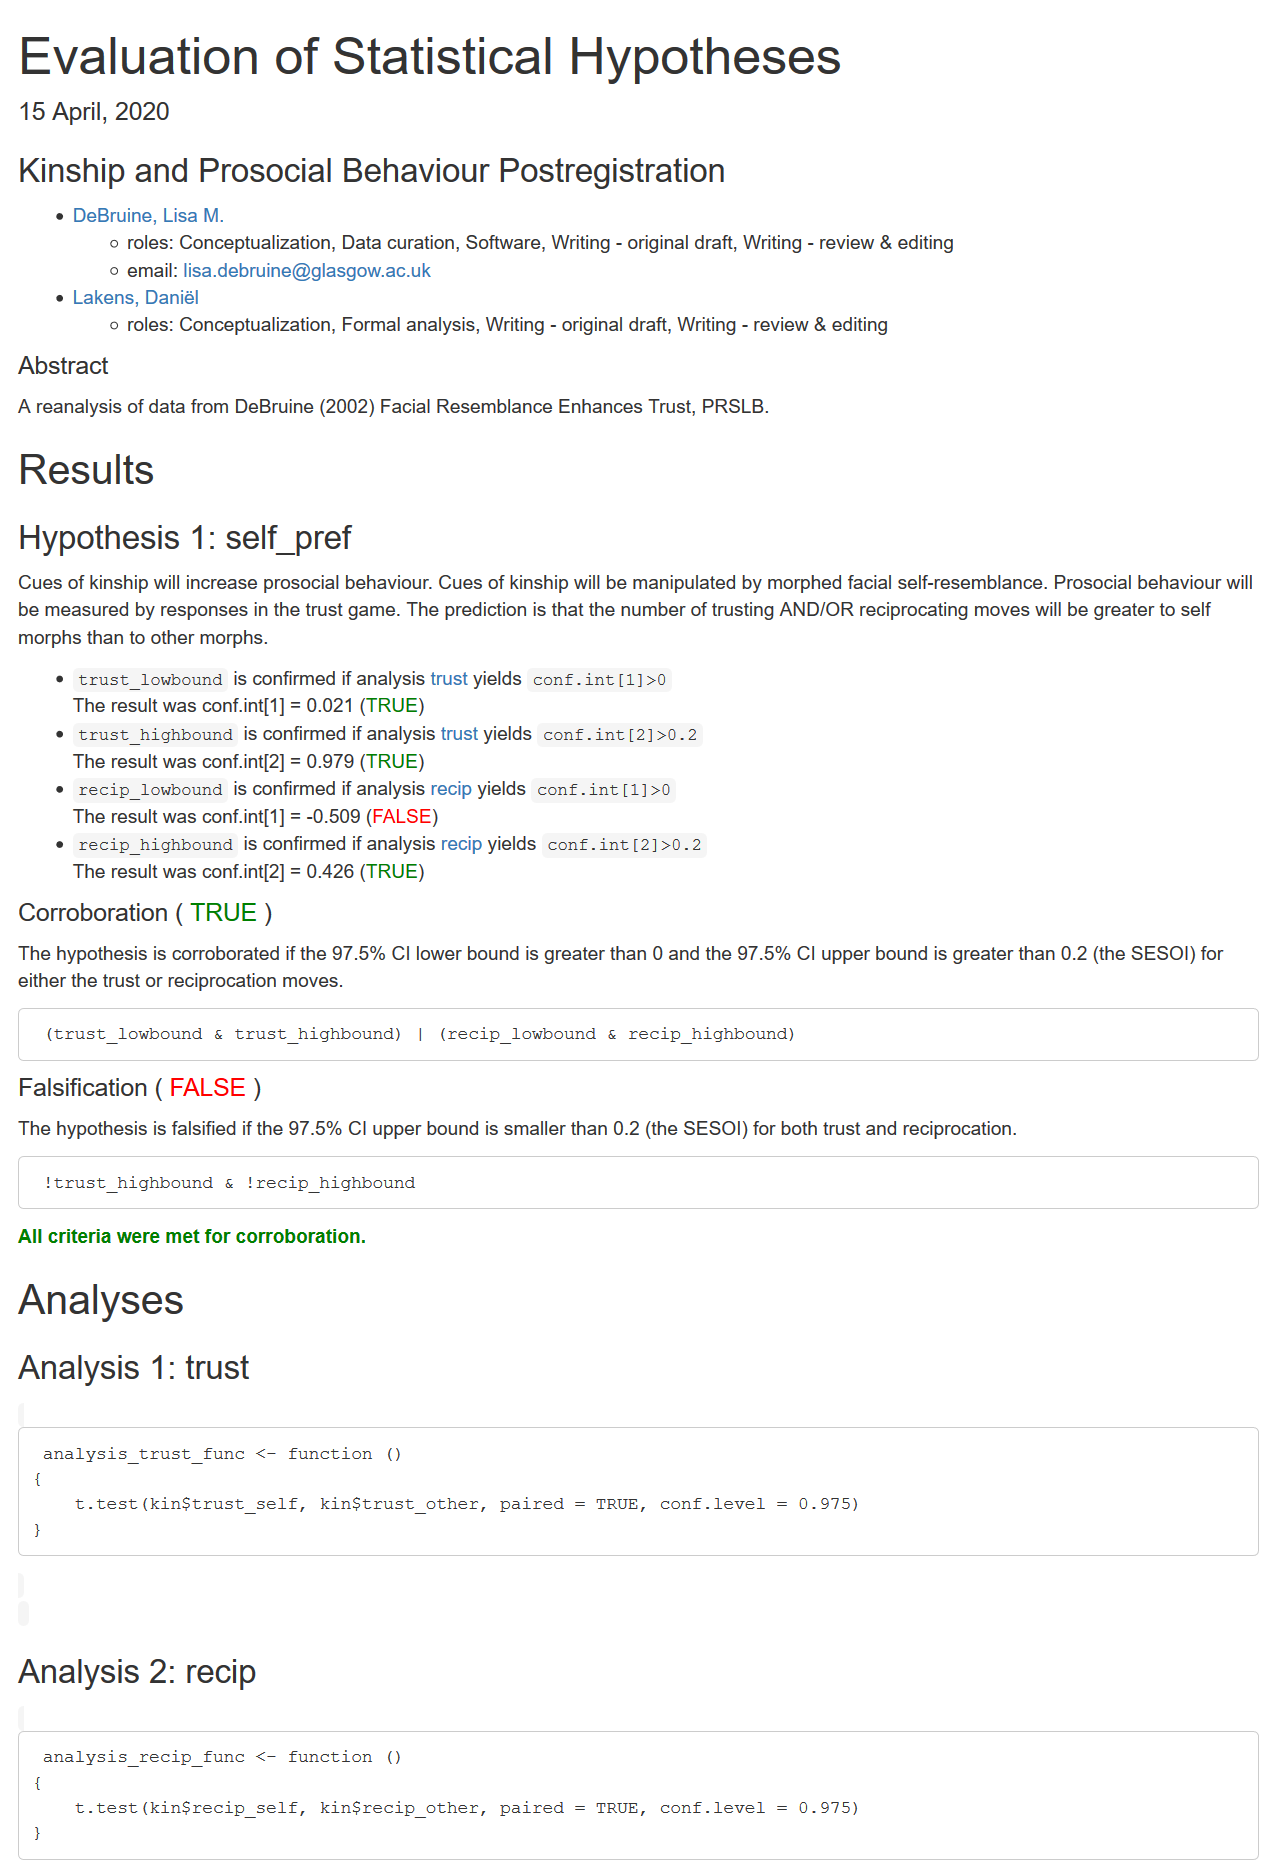
\includegraphics{images/output.png}
\caption{Example of machine readable output generated by scienceverse that shows the results and evaluation of the hypotheses. \label{fig1}}
\end{figure}

\hypertarget{benefits-of-machine-readability}{%
\subsection{Benefits of Machine Readability}\label{benefits-of-machine-readability}}

We believe the benefits of making statistical predictions machine readable are worth the extra effort. First, machine-readable hypotheses remove ambiguity about what researchers predict and which criteria must be met to conclude a statistical hypothesis is corroborated. Predictions are explicitly linked to the tests that are performed to evalaute if the prediction is corroborated or not. The exact test is specified, which prevents flexibility in the data analysis. Furthermore, specifying the criteria for corroboration or falsification explicitly prevents future researchers who will replicate the study from having to infer which results would corroborate or falsify the original finding. Although machine readable hypotheses might feel extremely rigid, it is possible to specify a range of sensitivity analyses across which the prediction should hold.

Another benefit of making statistical hypotheses machine readable is that many important aspects of the hypothesis test become accessible, findable, and usable. This will benefit researchers in the future. We can imagine a utopian future where meta-data files such as the example in Boxes 1 to 7 are accessible by browsing to a website that consists of the DOI, appended by /meta (e.g., \url{https://doi.org/10.1098/rspb.2002.2034/meta}). Researchers can access these files to load all the information that is available about statistical predictions. For example, when a completely reproducible workflow is used, and data can be accessed as part of the meta-data file, the meta-data file should be sufficient to easily calculate or access effect sizes from the performed statistical tests for meta-analyses.

While making hypothesis tests machine readable can obviously not ensure that statistical predictions are sensible or logically coherent, the process of writing a machine-readable statistical prediction could have a secondary benefit of providing a well-structured framework to think through and specify all important aspects of a statistical prediction. This might not be easy. Researchers might find it difficult to specify all required components in advance, or to specify the ranges of results that would corroborate or falsify a prediction. Sometimes a research idea is not yet well-specified enough to be tested in a confirmatory hypothesis test. Hypothesis tests are an extremely formalized procedure to make a decision whether a prediction is corroborated or not. If researchers realize they are actually not yet ready to make a falsifiable statistical prediction when creating a machine-readable hypothesis test, we would consider this a benefit as well, and we expect this to be a relatively common consequence of trying to formalize hypothesis tests.

\hypertarget{registered-reports-as-use-case}{%
\subsection{Registered Reports as Use Case}\label{registered-reports-as-use-case}}

We realize that several aspects of our proposal to make hypothesis tests machine readable sound futuristic. At the same time, we believe immediate use cases for machine-readable hypothesis tests already exist in the form of the Registered Report publication format (Chambers, 2019). Registered Reports require researchers to clearly specify their statistical prediction, and are developed to reduce flexibility in the statistical analyses. After Stage 1 review based on the introduction, methods, and analysis plan, researchers can receive an \enquote{in principle acceptance}. They then collect the data, and submit a Stage 2 Registered Report that includes the results and conclusion. Reviewers need to evaluate whether the analyses were conducted exactly as planned and whether conclusions follow from the predictions. This aspect of the peer review process is labor intensive and often still somewhat ambiguous, but could be automated if the statistical predictions were machine readable.

Scienceverse illustrates one possible workflow where after specifying the hypotheses at a Stage 1 submission, a machine-readable html report can be produced. This report looks similar to Figure 1, without any of the lines containing colored true or false evaluations of the predictions. When the data is collected, it can be added to the meta-data file generated at Stage 1, the preregistered analyses can then be run, and a human-readable report can be generated as in Figure 1. This should make it relatively easy for reviewers to compare planned and reported analyses.

\hypertarget{conclusions}{%
\subsection{Conclusions}\label{conclusions}}

Technological innovation makes it possible to communicate scientific findings in digital formats that allow for much easier re-use of scientific information contained in these digital files compared to traditional journal articles. As we move towards a time where researchers are expected to share their data in a way that is FAIR (findable, accessible, interoperable, and reusable), we believe it is feasible and beneficial to make the rest of research machine readable as well. We see machine-readable hypothesis tests as a logical development, with immediate benefits for the rigour of hypothesis tests. Increasing the accessibility of essential information related to hypothesis tests in scientific papers will also facilitate peer review, especially of Registered Reports, and facilitate meta-scientific research. Making statistical predictions machine readable will be an important next step towards a scientific literature that can be accessed not just visually, but also computationally.

\newpage

\hypertarget{author-contributions}{%
\subsection{Author Contributions}\label{author-contributions}}

Both authors conceptualized the main idea, LMD wrote the Scienceverse software, and both authors wrote and revised this manuscript.

\hypertarget{orcid-ids}{%
\subsection{ORCID iD's}\label{orcid-ids}}

Daniel Lakens 
\includegraphics{images/orcid.png} \url{https://orcid.org/0000-0002-0247-239X}

Lisa DeBruine 
\includegraphics{images/orcid.png} \url{https://orcid.org/0000-0002-7523-5539}

\hypertarget{acknowledgements}{%
\subsection{Acknowledgements}\label{acknowledgements}}

We would like to thank Leo Tiokhin and Peder Isager for feedback on an earlier draft of this manuscript, and attendants of a hackathon at the Society for the Improvement of Psychological Science for their enthusiastic reception of the ideas behind machine-readable hypotheses.

\hypertarget{declaration-of-conflicting-interests}{%
\subsection{Declaration of Conflicting Interests}\label{declaration-of-conflicting-interests}}

The author(s) declared that there were no conflicts of interest with respect to the authorship or the publication of this article.

\hypertarget{funding}{%
\subsection{Funding}\label{funding}}

LMD is supported by European Research Council grant \#647910. DL is funded by VIDI Grant 452-17-013 from the Netherlands Organisation for Scientific Research.

\hypertarget{open-practices}{%
\subsection{Open Practices}\label{open-practices}}

The code to reproduce this manuscript is available at \url{https://github.com/scienceverse/machine-readable} and the scienceverse R package is available from \url{https://github.com/scienceverse/scienceverse}.

\newpage

\hypertarget{references}{%
\section{References}\label{references}}

\begingroup
\setlength{\parindent}{-0.5in}
\setlength{\leftskip}{0.5in}

\hypertarget{refs}{}
\leavevmode\hypertarget{ref-arslan2019}{}%
Arslan, R. C. (2019). How to automatically document data with the codebook package to facilitate data reuse. \emph{Advances in Methods and Practices in Psychological Science}, \emph{2}(2), 169--187. \url{https://doi.org/10.1177/2515245919838783}

\leavevmode\hypertarget{ref-chambers2019}{}%
Chambers, C. (2019). What's next for registered reports? \emph{Nature}, \emph{573}, 187--189. \url{https://doi.org/10.1038/d41586-019-02674-6}

\leavevmode\hypertarget{ref-debruine2002}{}%
DeBruine, L. M. (2002). Facial resemblance enhances trust. \emph{Proceedings of the Royal Society of London. Series B: Biological Sciences}, \emph{269}, 1307--1312. \url{https://doi.org/10.1098/rspb.2002.2034}

\leavevmode\hypertarget{ref-dienes2019}{}%
Dienes, Z. (2019). How do I know what my theory predicts? \emph{Advances in Methods and Practices in Psychological Science}, \emph{2}(4), 364--377. \url{https://doi.org/10.1177/2515245919876960}

\leavevmode\hypertarget{ref-lakatos1978}{}%
Lakatos, I. (1978). \emph{The methodology of scientific research programmes: Volume 1: Philosophical papers.} Cambridge University Press.

\leavevmode\hypertarget{ref-lakens2018}{}%
Lakens, D., Scheel, A. M., \& Isager, P. M. (2018). Equivalence testing for psychological research: A tutorial. \emph{Advances in Methods and Practices in Psychological Science}, \emph{1}(2), 259--269. \url{https://doi.org/10.1177/2515245918770963}

\leavevmode\hypertarget{ref-neyman1933}{}%
Neyman, J., Pearson, E. S., \& Pearson, K. (1933). IX. On the problem of the most efficient tests of statistical hypotheses. \emph{Philosophical Transactions of the Royal Society of London. Series A, Containing Papers of a Mathematical or Physical Character}, \emph{231}(694-706), 289--337. \url{https://doi.org/10.1098/rsta.1933.0009}

\endgroup

\end{document}
